\chapter{Concept}

\section{Overview}

At the beginning the basic hardware setup was decided to be based on a Turtlebot 2 with an rigidly mounted additional RGBD-camera. This reduces the complexity of the problem as only movement of the whole robot in two dimensional space is possible with this setup. Assuming not too cluttered environments this setup should be sufficient for most search tasks.

Using visual information for object detection was an obvious choice. As the usage of commonsense knowledge was the main intention behind this work a general out of the box solution was preferred over a specialized handcrafted solution. Computer vision challenges for object detection and other computer vision tasks resulted in various available solutions for these problems to choose from. As object detection systems using color images as input and bounding boxes of detected objects as output were the only systems with a sufficient number of detectable object classes and reasonable accuracy while not being too resource-demanding for the used hardware such a system was chosen. This left the problem of getting from the bounding boxes in the image to a three dimensional representation needed for the search. The depth information of the RGBD-camera was used to project the detections into 3D space and an approach similar to occupancy grid mapping was used to merge the detections of different images into a three dimensional object probability map.

To make the search more intelligent the concept of a room was implemented. Like humans the robot can assign a type to every room, e.g. kitchen. As there is a high correlation between the type of a room and the objects located in this room the classification of a room and its usage to guide the object search is highly beneficial. In this work the classification of rooms was done using a neural network for place classification and also the objects found in this room were used. As in some cases one room consists of areas of different rooms types, e.g. a kitchenette in an office room, the room is split into a grid of cells holding the probability distribution of the cell being of a certain room type over all room types.

The fact that indoor environments can be segmented into rooms is used in the representation of the environment. A hybrid map consisting of a topological map depicting the room structure and metric maps for every room combine the advantages of both map types. This structure is easy to maintain as rooms are only connected by narrow doorways which can be detected reliably.

This structure is also the basis for the planning. A high-level planner working on the topological map chooses the next room to search based on the expected object probabilities and search times in the rooms and the expected travel times between the rooms. A low-level planner plans the tasks within the room like room exploration and search. This greatly simplifies the planning problem and should still lead to good results as the object probability is correlated to the room type.

Fig bla1 shows the 

% In the early phase we had to make some fundamental decisions regarding the hardware and the basic concept. 
% Firstly a Turtlebot was chosen as the basic robot setup. To improve the navigation capabilities we replaced the Microsoft Kinect of the standard Turtlebot setup with a far more accurate laser scanner. Visual object detection was the obvious choice, therefore a camera was mounted. We choose an ASUS XTion RGBD-camera because the additional depth information could be used for 3D mapping and obstacle detection. \newline
% Another fundamental decision was to heavily use the fact that indoor environments can be segmented into rooms. This makes the use of a hybrid map to represent the environment very appealing. Every room is a node in a topological map and contains, beside other information, a metric map. The doorways between the rooms are the edges in the topological map. This representation is also used in the planning process, which is split into a high-level planning and a low-level planning. The high-level planning is used to select the next room based on the topological map and the low-level planning has then only to consider the current room. \newline
% As the focus was on the usage of commonsense knowledge the use of a universal object detection instead of a specialized one was intended. This led to the decision to use a convolutional nerual  network for object detection. As the accuracy of those CNNs is still not so great and the number of possible objects in a room is quiet high object tracking is most likely infeasible. Therefore the use of an approach similar to occupancy grid mapping to generate a probability distribution for objects of a specific class was decided. \newline
% The use of commonsense knowledge regarding the correlation between room type and object probability can boost the search efficiency. As a room might have different part, e.g. a kitchenette in a living room, a grid representing the probability distribution of a cell being of a certain room is generated and used to improve the probability distribution of object occurances.
% 
% Fig blabla shows the resulting structure or the hybrid map.  

\subsection{Hardware}

The robot used in this work is a modified version of the Turtlebot 2. The Yujin Kobuki base of the Turtlebot is a differential drive base with an odometry, amended by a gyroscope. The maximum translational velocity of this base is 0.7 m/s, the maximum rotational velocity is 180°/s and the maximum payload is 5 kg. 

For accurate localization and 2D mapping a Hokuyo laser range finders (LIDAR) is mounted on the base. The specified range is from 0.02 m to 4 m with an accuracy of $\pm10$ mm and the angular range is from -120° to 120° with a resolution of 0.36°. The LIDAR scans at a rate of 10 Hz.

The main camera for object detection, place classification and 3D mapping is an ASUS Xtion PRO LIVE RGBD-camera mounted at a height of about 1m facing slightly downwards. The camera takes color images and depth images at a rate of 30 Hz with a resolution of 640x480. The field of view is 58° horizontally and 45° vertically. The range of the depth measurements is specified with 0.8 m to 3.5 m, though experiments showed a minimum range of about 0.55 m. The accuracy of the depth image depends on many factors, especially on the distance and is somewhere around $\pm$5 cm (TODO genauer wert und referenz).\newline
For the detection of doorways another ASUS Xtion PRO LIVE was added looking upwards.

A Clevo notebook is mounted on the robot running the complete software with a $4^{th}$ generation Intel i7 quadcore CPU running at 2.4 GHz, 8 GB DDR3 RAM and a NVidia Geforce GT 750M GPU with 2 GB memory. 

\begin{figure}
  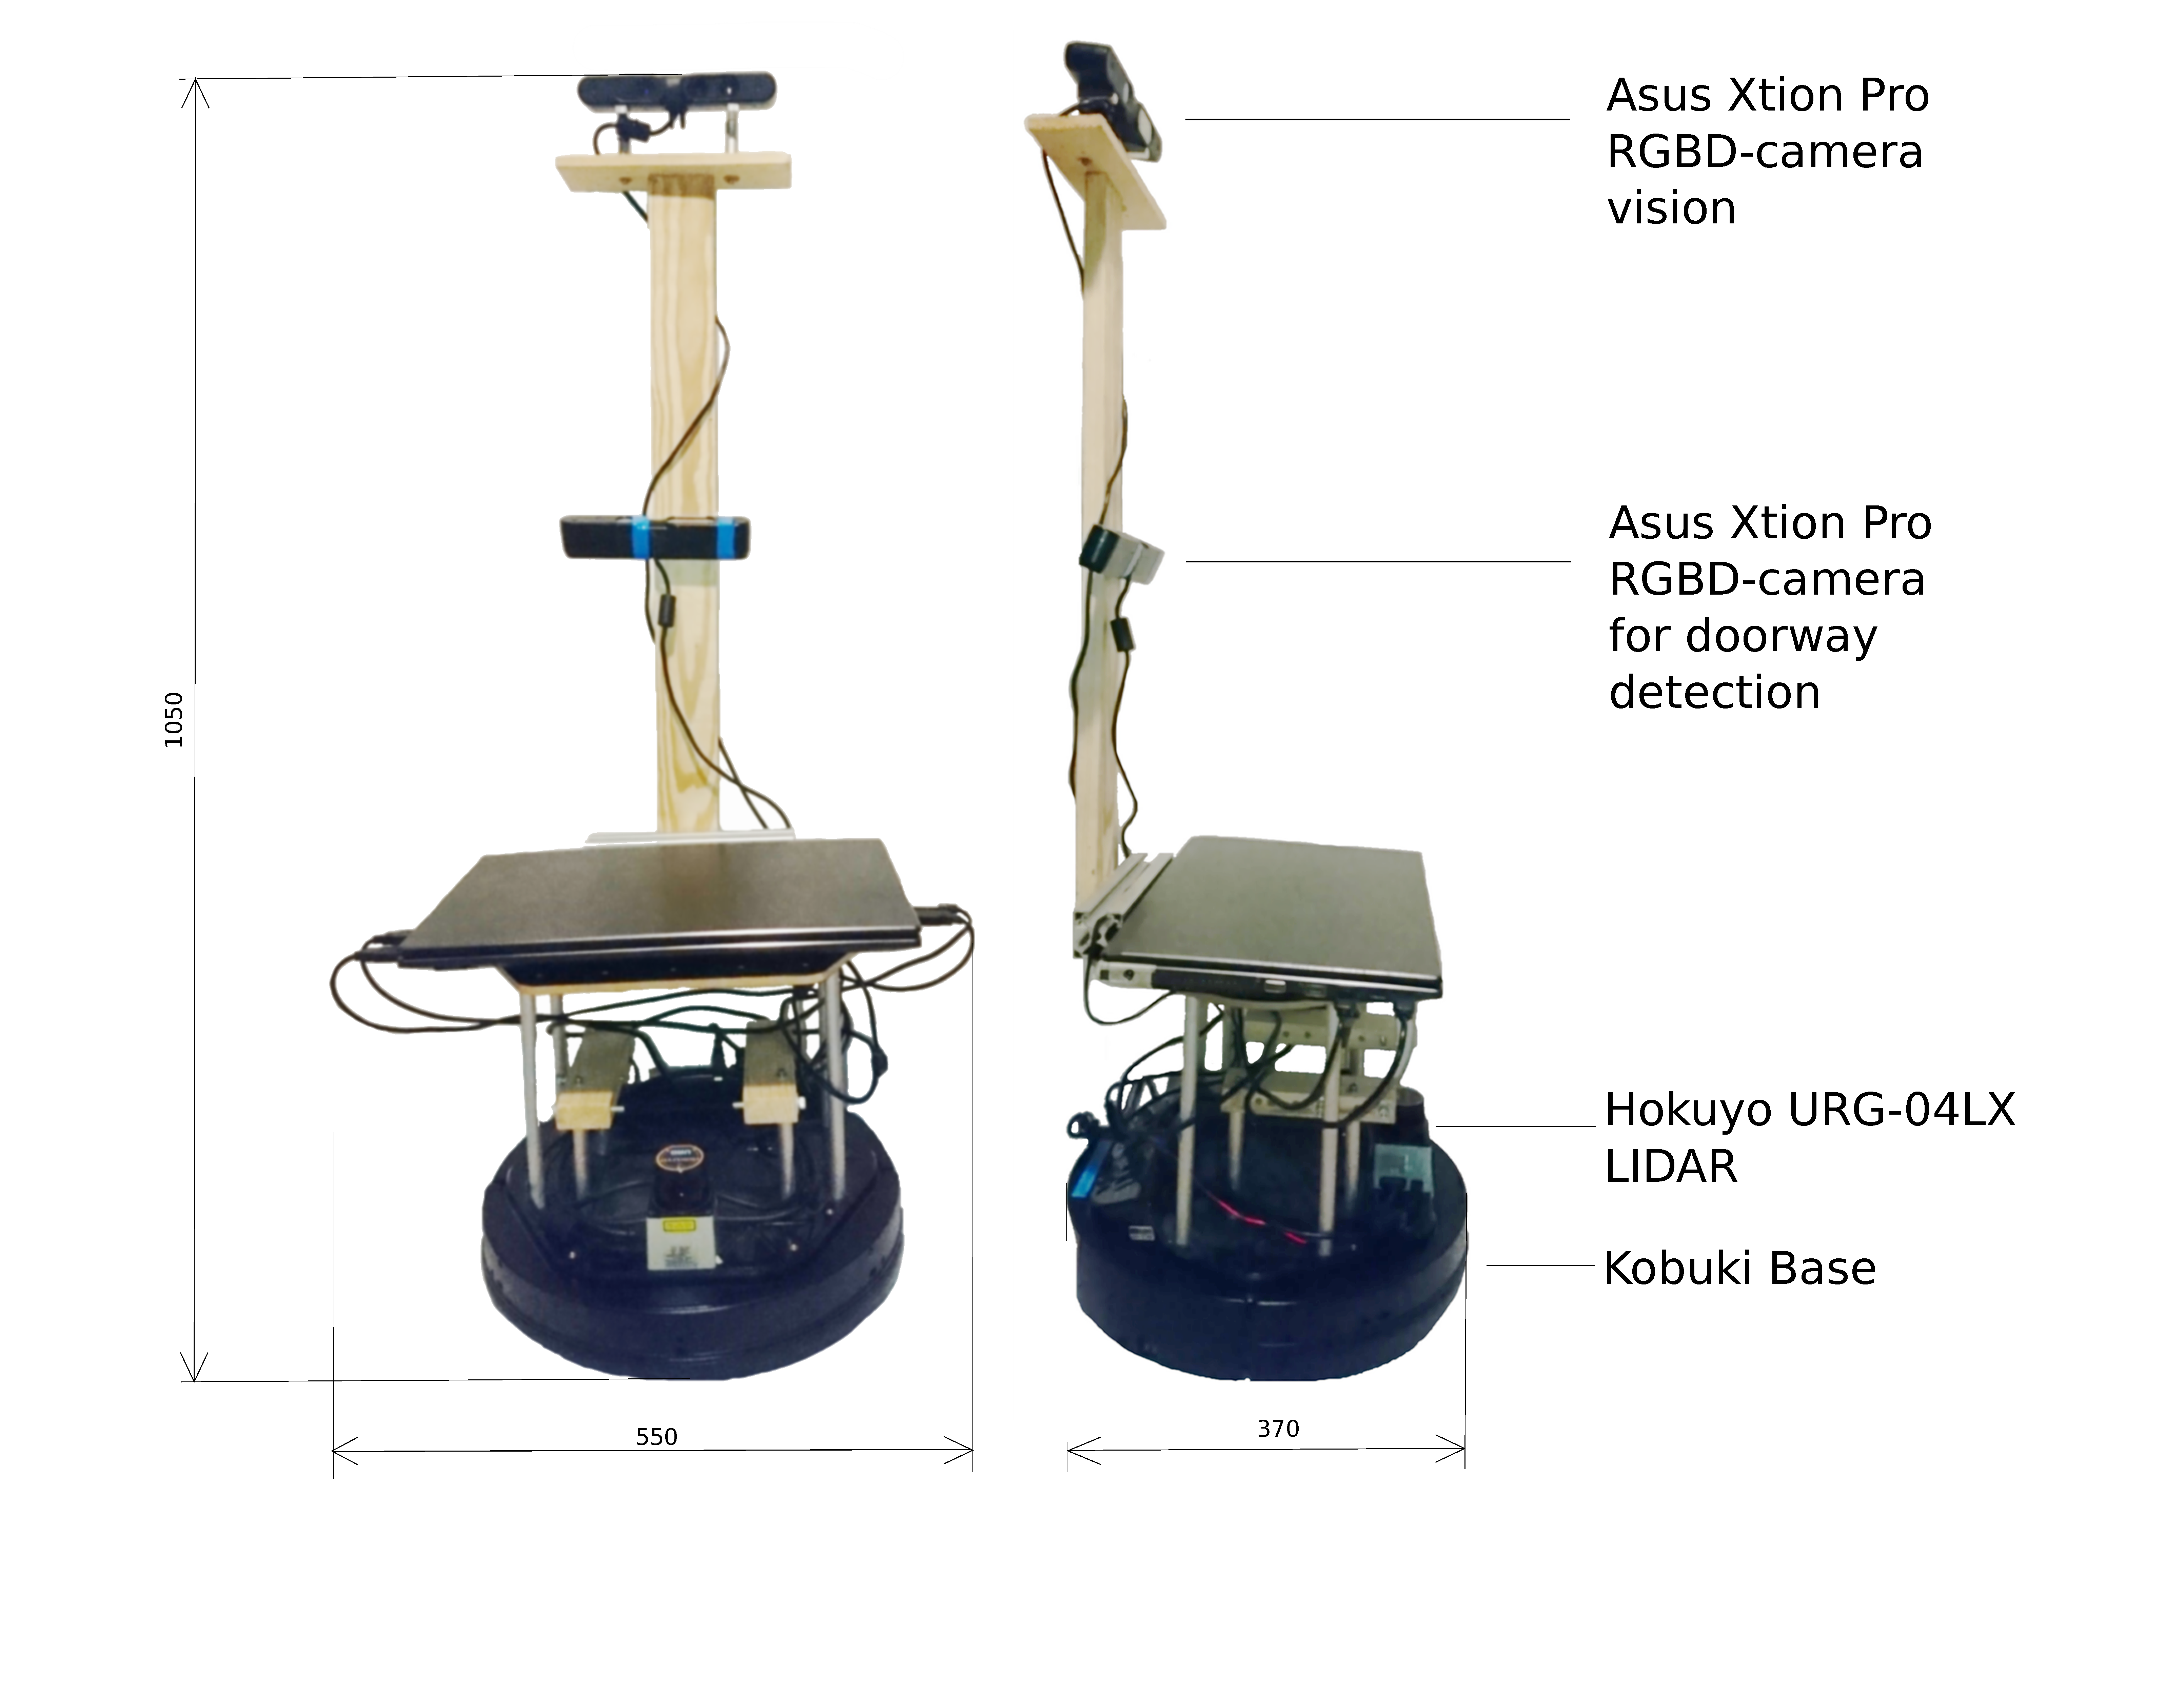
\includegraphics[width=1.02\textwidth,trim={0 5cm 0 0},clip]{figures/front_and_side.pdf}
  \caption{Robot setup in front and side view with labels of most important parts}
\end{figure}
